\documentclass[a4paper,11pt]{article}
\usepackage[T1]{fontenc}
\usepackage[utf8]{inputenc}
\usepackage{lmodern}
\usepackage[english]{babel}
\usepackage{subcaption}
\usepackage{graphicx}
\usepackage{listings}
\usepackage{color}
\usepackage{hyperref}
\usepackage{titlesec}

\titleformat{\section}{\normalfont\Large\bfseries}{Question \thesection}{1em}{}
\renewcommand{\thesubsection}{\thesection.\alph{subsection}}

\definecolor{dkgreen}{rgb}{0,0.6,0}
\definecolor{gray}{rgb}{0.5,0.5,0.5}
\definecolor{mauve}{rgb}{0.58,0,0.82}

\lstset{frame=tb,
  language=Python,
  aboveskip=3mm,
  belowskip=3mm,
  showstringspaces=false,
%   columns=flexible,
  basicstyle={\small\ttfamily},
  numbers=left,
%   frame=single,
  morekeywords={mean,std},
  numberstyle=\tiny\color{gray},
  keywordstyle=\color{blue},
  commentstyle=\color{dkgreen},
  stringstyle=\color{mauve},
  breaklines=true,
  breakatwhitespace=true,
  tabsize=3
}

\title{Computer vision - Homework 1}
\author{Nicolas Six}

\begin{document}

\maketitle

\section{Edges detection}

\begin{figure}[h!]
  \begin{center}
    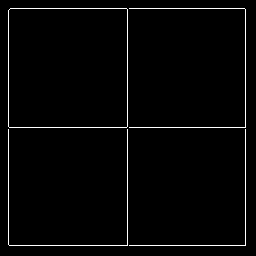
\includegraphics[width=0.35\linewidth]{{../Images/ps1-1-a}.png}
    \caption{Edge image}
  \end{center}
\end{figure}

\section{Hough line detection}
\paragraph{}
The accumulator is a square array of size $d$, with $d$ the source image's diagonal length. One of the dimension of the accumulator must be of size $d$ as the line are described in a polar way. We chose to code the angle on the same number of value to keep a consistent precision between them.

\begin{figure}[h!]
  \begin{center}
    \begin{subfigure}[t]{0.49\columnwidth}
      \centering
      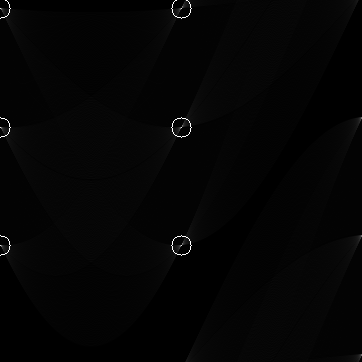
\includegraphics[width=.7\linewidth]{{../Images/ps1-2-a}.png}
      \caption{Accumulator}
    \end{subfigure}
    \begin{subfigure}[t]{0.49\columnwidth}
      \centering
      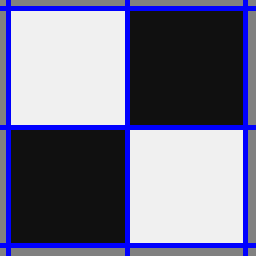
\includegraphics[width=.7\linewidth]{{../Images/ps1-2-b}.png}
      \caption{Line detected}
    \end{subfigure}
    \caption{question 2 results}
  \end{center}
\end{figure}

\section{Line on noisy image}
\subsection{Smoothing}
\begin{figure}[h!]
  \begin{center}
    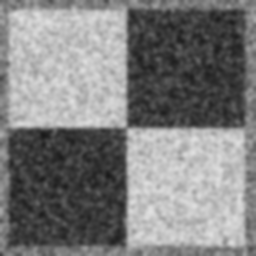
\includegraphics[width=0.35\linewidth]{{../Images/ps1-3-a}.png}
    \caption{Smoothed image}
  \end{center}
\end{figure}

\subsection{Edges detection}
\begin{figure}[h!]
  \begin{center}
    \begin{subfigure}[t]{0.49\columnwidth}
      \centering
      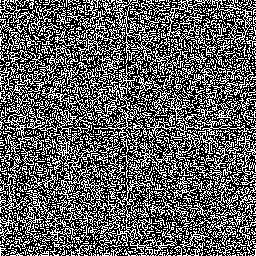
\includegraphics[width=.7\linewidth]{{../Images/ps1-3-b-1}.png}
      \caption{Edges on noisy image}
    \end{subfigure}
    \begin{subfigure}[t]{0.49\columnwidth}
      \centering
      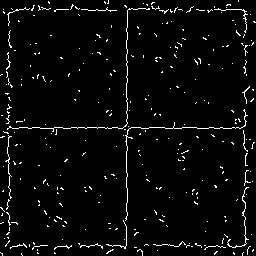
\includegraphics[width=.7\linewidth]{{../Images/ps1-3-b-2}.png}
      \caption{Edges on smoothed image}
    \end{subfigure}
    \caption{Edges detected}
  \end{center}
\end{figure}

\subsection{Hough lines}
\begin{figure}[h!]
  \begin{center}
    \begin{subfigure}[t]{0.49\columnwidth}
      \centering
      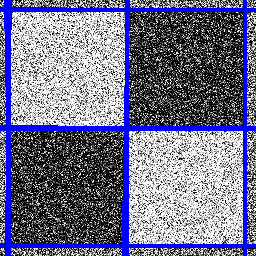
\includegraphics[width=.7\linewidth]{{../Images/ps1-3-c-1}.png}
      \caption{Accumulator}
    \end{subfigure}
    \begin{subfigure}[t]{0.49\columnwidth}
      \centering
      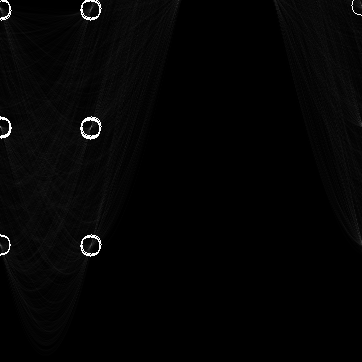
\includegraphics[width=.7\linewidth]{{../Images/ps1-3-c-2}.png}
      \caption{Line detected}
    \end{subfigure}
    \caption{question 3.c results}
  \end{center}
\end{figure}
\paragraph{}
To have this result we had to adjust the threshold of the line detection as well as smoothing to prevent the Hough method to find unreal lines.

\section{Easy real image - lines}
\subsection{Smoothing}
\begin{figure}[h!]
  \begin{center}
    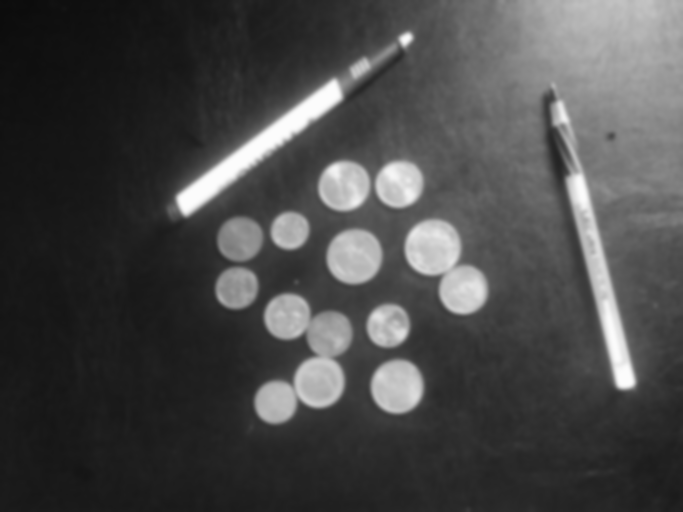
\includegraphics[width=0.35\linewidth]{{../Images/ps1-4-a}.png}
    \caption{Smoothed image}
  \end{center}
\end{figure}

\subsection{Edges}
\begin{figure}[h!]
  \begin{center}
    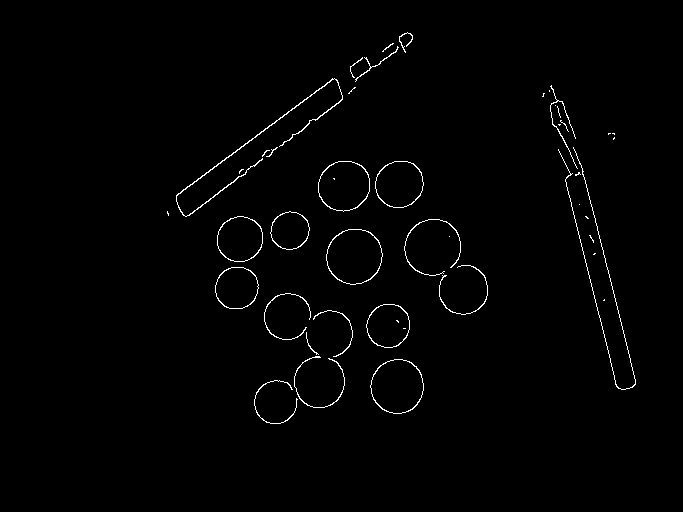
\includegraphics[width=0.35\linewidth]{{../Images/ps1-4-b}.png}
    \caption{Edges image}
  \end{center}
\end{figure}

\subsection{Hough line detection}
\begin{figure}[h!]
  \begin{center}
    \begin{subfigure}[t]{0.49\columnwidth}
      \centering
      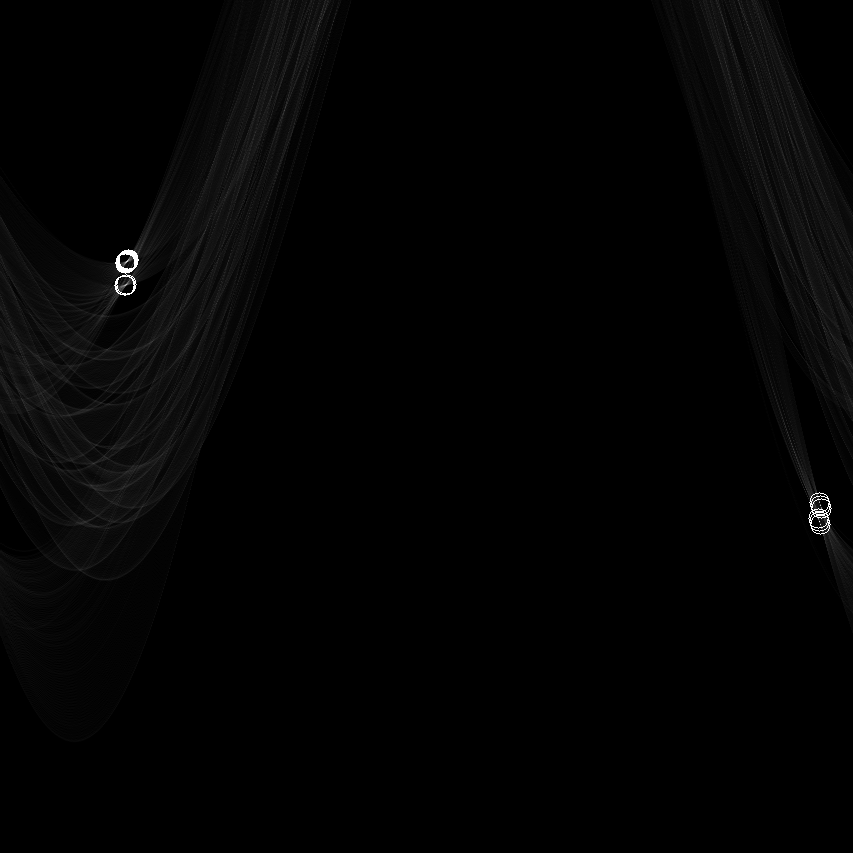
\includegraphics[width=.7\linewidth]{{../Images/ps1-4-c-1}.png}
      \caption{Accumulator}
    \end{subfigure}
    \begin{subfigure}[t]{0.49\columnwidth}
      \centering
      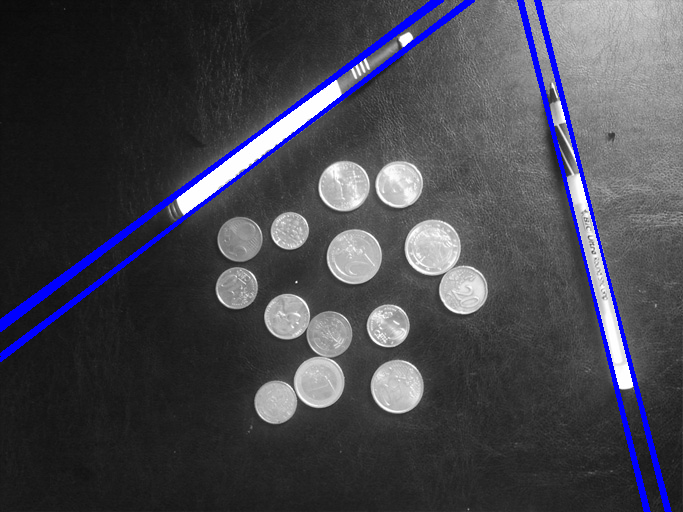
\includegraphics[width=.7\linewidth]{{../Images/ps1-4-c-2}.png}
      \caption{Line detected}
    \end{subfigure}
    \caption{question 4.c results}
  \end{center}
\end{figure}
\paragraph{}
This question needed very little adjustment of the the threshold mostly.


\section{Circles - easy}
\begin{figure}[h!]
  \begin{center}
    \begin{subfigure}[t]{0.49\columnwidth}
      \centering
      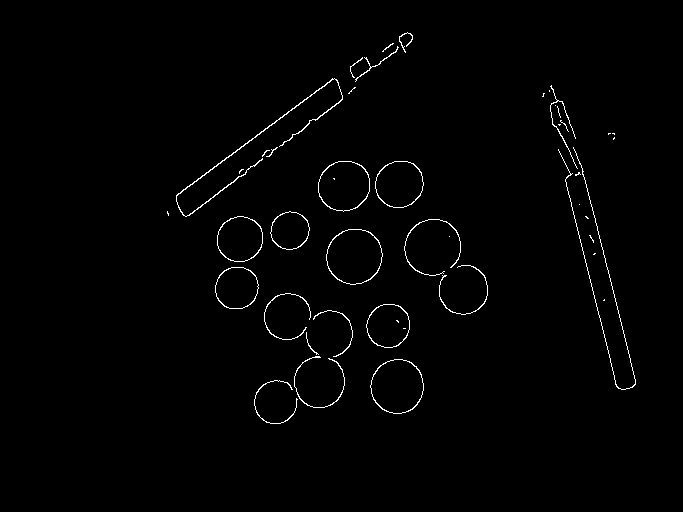
\includegraphics[width=.7\linewidth]{{../Images/ps1-5-a-1}.png}
      \caption{Edges image}
    \end{subfigure}
    \begin{subfigure}[t]{0.49\columnwidth}
      \centering
      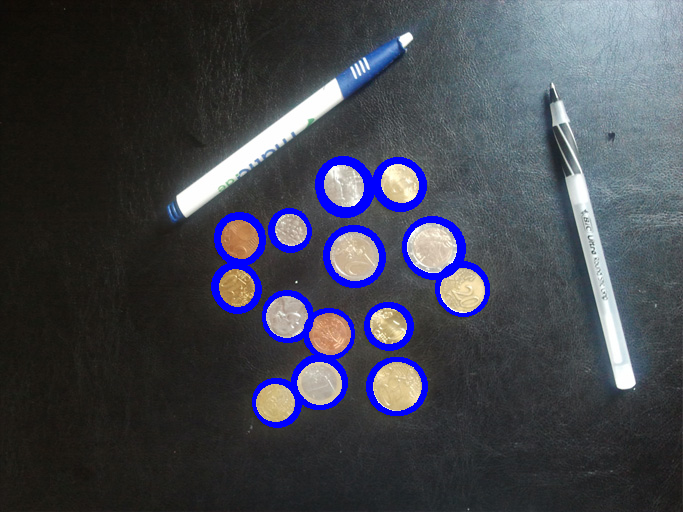
\includegraphics[width=.7\linewidth]{{../Images/ps1-5-a-2}.png}
      \caption{Circle detected}
    \end{subfigure}
    \caption{question 5 results}
  \end{center}
\end{figure}
\paragraph{}
The Hough circle detection is very similar to the line detection, but with a 3D accumulator. To remove a nest for loop, we used the openCV function to draw a circle. This trick worsen the theoretical complexity but is more effective in python as both the circle draw and the plan addition are implemented in C.

\begin{lstlisting}
for x, y in zip(edges_points_x, edges_points_y):
    for r in range(min_radius, max_radius):
        plane = np.zeros((h, w))
        cv2.circle(plane, (x, y), r, (1, 0, 0), 1)
        acc[r - min_radius] += plane
\end{lstlisting}

\section{More realistic images - Lines}

\subsection{Line finder}

\begin{figure}[h!]
  \begin{center}
    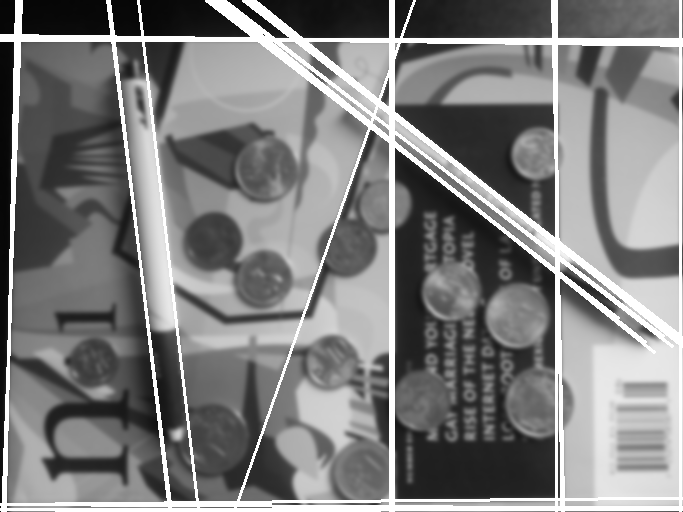
\includegraphics[width=0.35\linewidth]{{../Images/ps1-6-a}.png}
    \caption{Line found}
  \end{center}
\end{figure}

\subsection{Problems present}
\paragraph{}
Our main problem here, is that even if all the pen's lines are found other lines from the background are too. But, those background lines are sharper and longer than the one of the pens and thus thresholding is not enough to select only the pens lines.


\subsection{Line finder - Bis}

\begin{figure}[h!]
  \begin{center}
    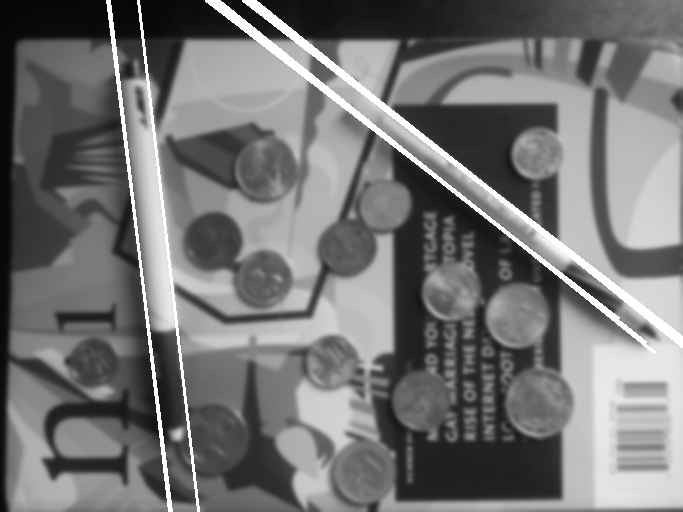
\includegraphics[width=0.35\linewidth]{{../Images/ps1-6-c}.png}
    \caption{Line found}
  \end{center}
\end{figure}

\section{More realistic images - Circles}

\subsection{Circle finder}
\begin{figure}[h!]
  \begin{center}
    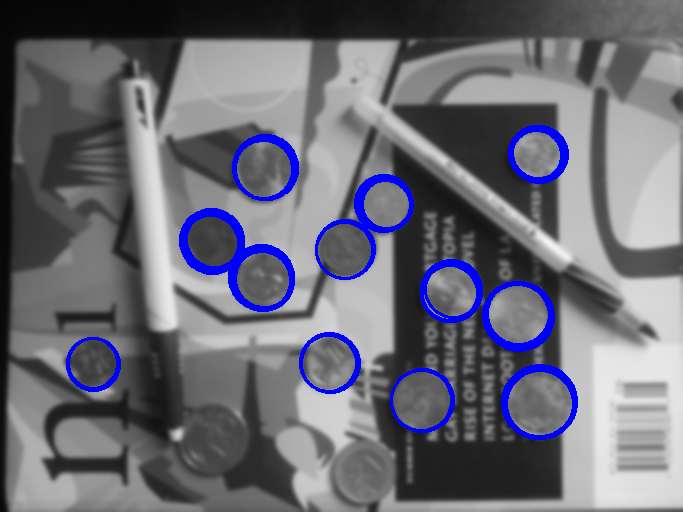
\includegraphics[width=0.35\linewidth]{{../Images/ps1-7-a}.png}
    \caption{Circles found}
    \label{q7}
  \end{center}
\end{figure}

\subsection{Face alarm}

As it can be seen an Figure \ref{q7}, their are no false alarm, but only twelve of the fourteen circles are found. To achieve that result, we mainly fine tuned the existing parameters such as the edges detection threshold and circle detection threshold as well as the maximum and minimum size of the circle. Another approach that we tried is to divide the number of vote for a circle by the radius of the given circle. The goal here is transform the threshold from the number of vote for a center, to the proportion of point of the circle voting for this center, and so have a threshold that manage both big and small radius.

\section{Distortion}

\subsection{Line and Circles}
\begin{figure}[h!]
  \begin{center}
    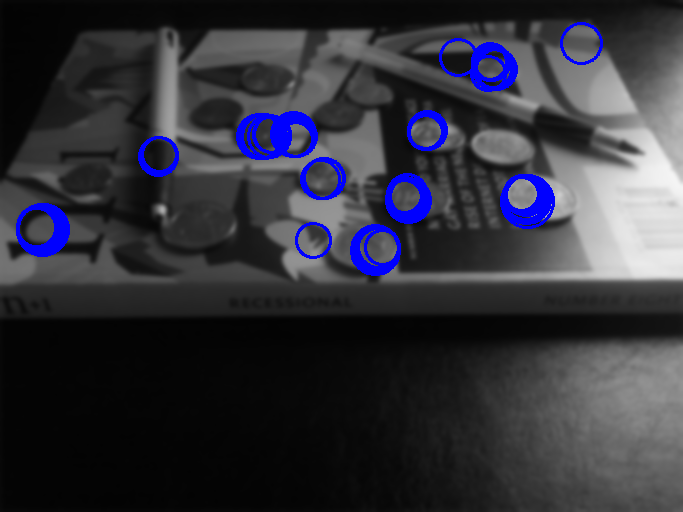
\includegraphics[width=0.35\linewidth]{{../Images/ps1-8-a}.png}
    \caption{Circles and lines found}
  \end{center}
\end{figure}

\subsection{How to fix circle problem}
\paragraph{}
The most reliable way to fix the circle problem is to transform our circle finder into an ellipse finder. Doing so, we will still be able to find the wanted circles even when not exactly taken from above.

One way to do so is to add two others parameters, for example the second radius of the ellipsis and its orientation and have an 5D accumulator. If this solution probably work, it's far from an optimal solution in term of computation complexity. This complexity can probably be reduced using the local gradient, but it may still be time consuming. Another simplification can be that every circles are distorted in the same way, such as the angle of the ellipsis and the rapport between the two radius are constant. By fixing those parameters we came back to the same complexity than the classic circle finder.

\subsection{Fixing circle problem}
\paragraph{}
But we do not chose to apply such a strategy to fund the circles. Instead we chose a more lazy way in term of implementation. As we know that the only problem we have to solve is that the image do not came from the right angle, but the plan on the image is still a plane. We can take advantage of the OpenCV function to transform the image such as circle look like circle again, in other word, transform the picture to make it look (a bit) like it was taken from above. The result is displayed on Figure \ref{cheat1}.

\begin{figure}[h!]
  \begin{center}
    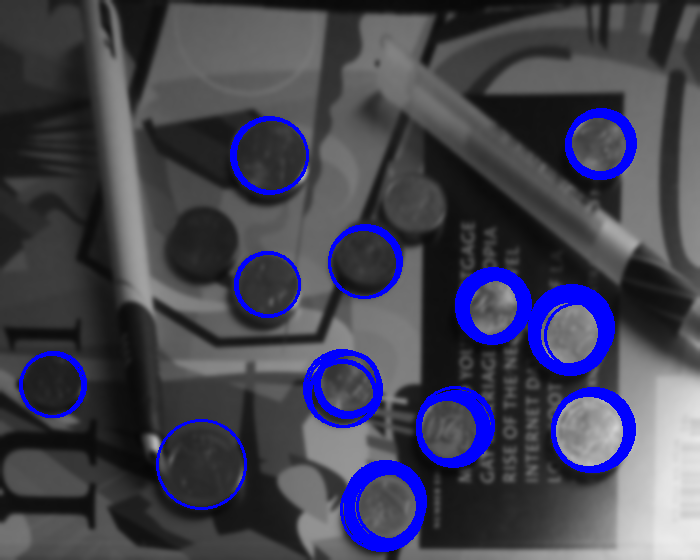
\includegraphics[width=0.35\linewidth]{{../Images/ps1-8-c-1}.png}
    \caption{Circles found}
    \label{cheat1}
  \end{center}
\end{figure}

\paragraph{}
It is easy to argument that the picture doesn't look like the original one, which can by corrected by applying the inverse transform (Figure \ref{cheat2}), and by adding back the previously discarded pixels (Figure \ref{cheat3}).

\begin{figure}[h!]
  \begin{center}
    \begin{subfigure}[t]{0.49\columnwidth}
      \centering
      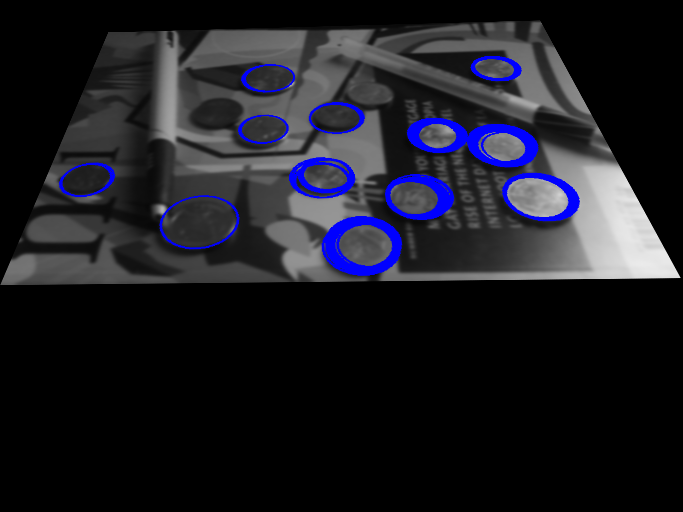
\includegraphics[width=.7\linewidth]{{../Images/ps1-8-c-2}.png}
      \caption{Back in the original perspective}
      \label{cheat2}
    \end{subfigure}
    \begin{subfigure}[t]{0.49\columnwidth}
      \centering
      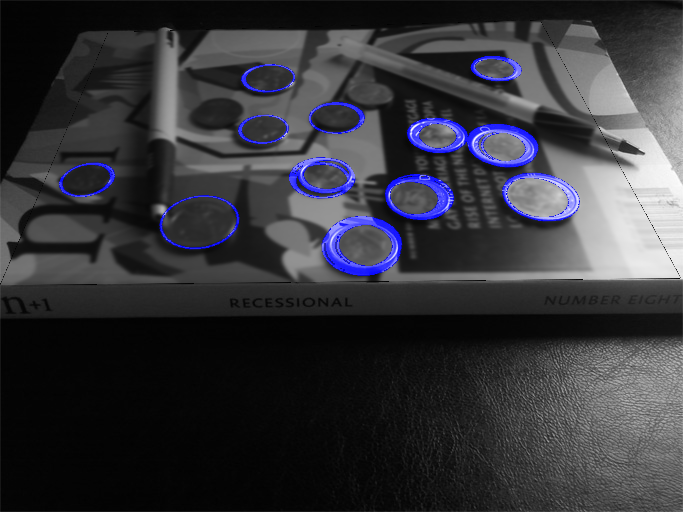
\includegraphics[width=.7\linewidth]{{../Images/ps1-8-c-3}.png}
      \caption{Add original background}
      \label{cheat3}
    \end{subfigure}
    \caption{Distortion detection Final result}
  \end{center}
\end{figure}

\end{document}

